\documentclass{article}
\usepackage{times}
\usepackage[english,russian]{babel}
\usepackage[utf8]{inputenc}
\usepackage{dirtytalk}
\usepackage[a4paper, total={6in, 8in}]{geometry}
\usepackage{graphicx}
\usepackage{hyperref}


\graphicspath{ {./img/} }

\begin{document}
\title{BlockChain. Ethereum.}

\date{\today}
\maketitle

\say{Всегда пишите код так, будто сопровождать его будет склонный к насилию психопат, который знает, где вы живете.
— Martin Golding}


\section{Введение}

\subsection{Что такое блокчейн?}

Блокчейн – это криптографически безопасная транзакционная одноэлементная система с общим состоянием. Далеко не самое простое определение, не так ли? Давайте разобьем каждую составляющую этого определения на отдельные части.



\begin{itemize}
 \item «Криптографически безопасный» означает, что безопасность криптовалюты обеспечивается сложными математическими алгоритмами, которые практически невозможно обойти. Защита, выстроенная с помощью данных алгоритмов, представляет собой подобие файрвола: благодаря используемым алгоритмам обход системы безопасности практически невозможен (например, невозможно создание поддельных транзакций, уничтожение транзакций и т. д.).
 \item «Транзакционная одноэлементная система» означает, что существует только одно заданное состояние системы, благодаря которому происходят все транзакции, создаваемые в данной системе. Другими словами, для данной системы предусмотрено только одно состояние, которое является единственно верным.
 \item «С общим состоянием» означает, что состояние, заданное в системе, является общим и открытым для всех.
\end{itemize}

Таким образом, в платформе Эфириум реализуется приведенная выше парадигма блокчейна. 

\section{Теория}

\subsection{Парадигма блокчейна платформы Эфириум}

Блокчейн Эфириум является, по сути, системой состояния транзакций. В информатике такое понятие, как «система состояний» или «машина состояний» – это система, которая обрабатывает вводимую информацию и на основании последней преобразуется в новое состояние (Рис. 1). 

\begin{figure}
    \centering
    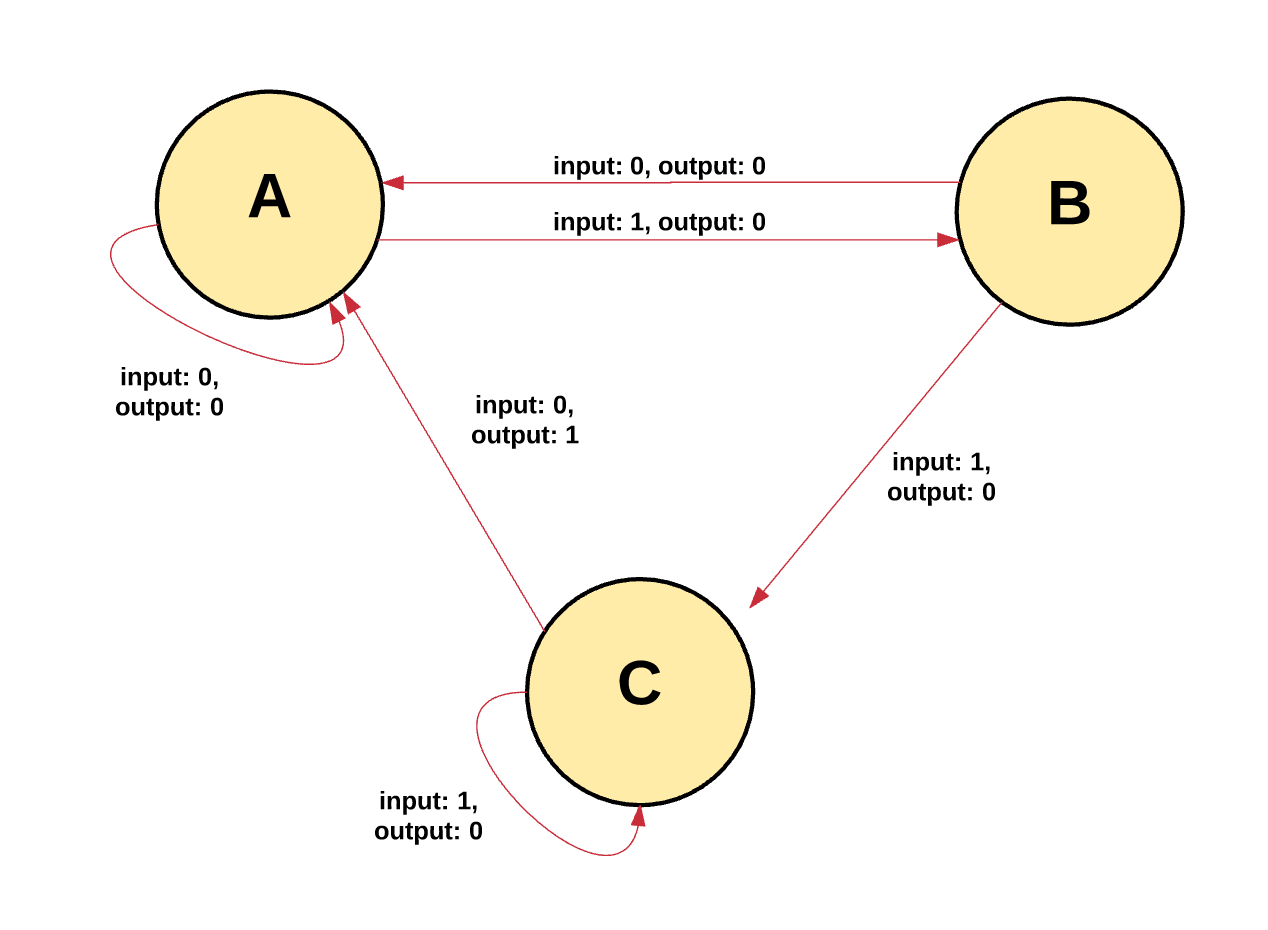
\includegraphics[scale=0.25]{scheme_1}
    \caption{Упрощенная схема работы блокчейна (машина состояний).}
    \label{fig:scheme_1}
\end{figure}

В машине состояний Эфириума все процессы начинаются с «первоначального состояния». Такое состояние представляет собой аналог нулевого состояния, в котором находится машина до того момента, как в ее сети начнут происходить какие-либо действия, связанные с транзакциями. Когда такие действия начнут происходить, первоначальное состояние заменяется на конечное, при этом в любой момент времени конечное состояние отображает текущее состояние Эфириума (Рис. 2).


\begin{figure}
    \centering
    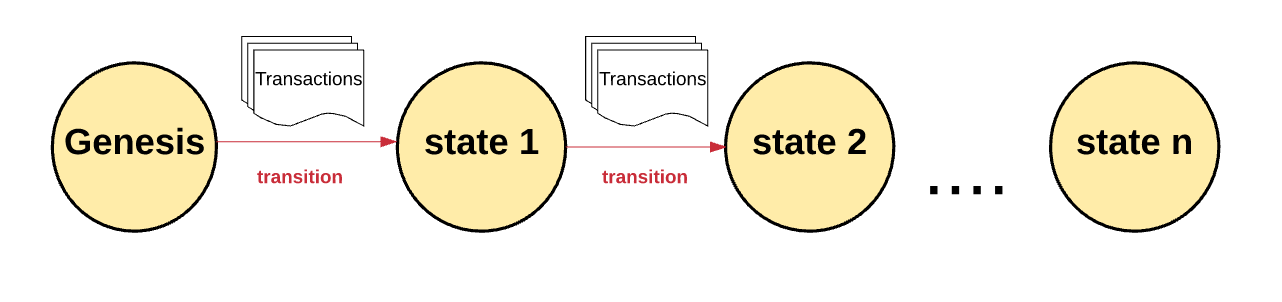
\includegraphics[scale=0.3]{scheme_2}
    \caption{Схема транзакций).}
    \label{fig:scheme_2}
\end{figure}


Состояние Эфириума имеет миллионы транзакций. Эти транзакции сгруппированы в «блоки». Блок содержит ряд транзакций, при этом каждый последующий блок соединен с предыдущим, благодаря чему обеспечивается своеобразная цепочка блоков (Рис. 3).


\begin{figure}
    \centering
    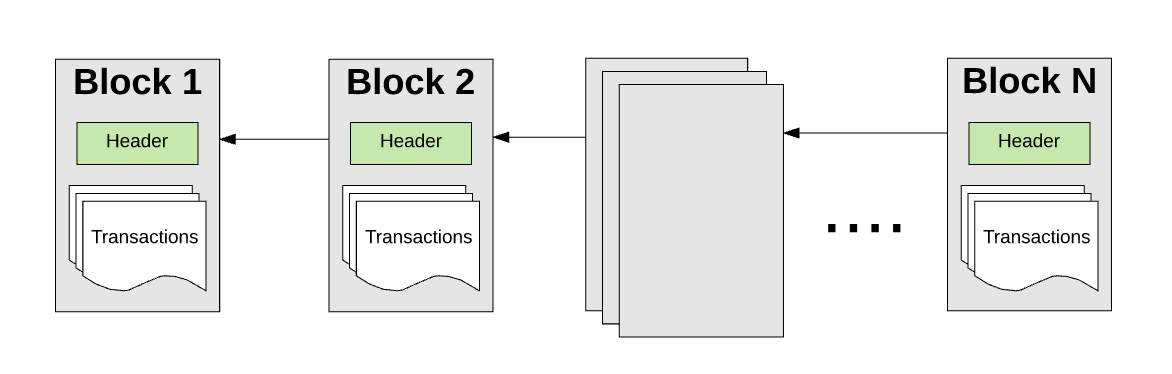
\includegraphics[scale=0.3]{scheme_3}
    \caption{Блоки тразакций.}
    \label{fig:scheme_3}
\end{figure}


Транзакция должна быть корректной, для того чтобы вызвать ее переход из одного состояния в другое. Транзакция считается корректной только тогда, когда она прошла процесс проверки – так называемый «майнинг». Майнинг — это когда группа узлов (компьютеров) расходует свои вычислительные ресурсы для создания блока корректных транзакций.

Любой узел в сети, объявляющий себя майнером, может попытаться создать и проверить блок транзакций. Распространенным опытом является попытки множества майнеров одновременного создания и проверки блока транзакций. Каждый майнер предоставляет свое математическое «доказательство» при отправке блока в блокчейн, и это доказательство выступает в роли своеобразной гарантии: в случае если доказательство существует, транзакции в блоке считаются корректными.

Майнер должен предоставить свое математическое доказательство быстрее, чем это сделает любой другой конкурент, для того чтобы его блок был добавлен в основной блокчейн. Процесс проверки каждого блока, который заключается в предоставлении майнером своего математического доказательства, называется «доказательством работы».

Майнер, который обосновывает новый блок, получает определенное вознаграждение за выполнение этой работы. О каком вознаграждении идет речь? В блокчейне Эфириума используется встроенный цифровой токен, который носит название «эфир» (от англ. ether— «эфир»). Каждый раз, когда майнер обосновывает свой блок транзакций, создается новый токен или новый эфир, а майнер получает вознаграждение за его создание.

Тогда, у вас может возникнуть вполне логичный вопрос: где гарантия того, что каждый майнер будет придерживается только одной цепочки блоков? Как мне убедиться в том, что другая команда майнеров не решит создать свою собственную цепочку блоков?

В самом начале данной статьи мы уже приводили такое понятие как «транзакционная одноэлементная система с общим состоянием». Исходя из такого определения можно сделать вывод, что не бывает двух и более корректных текущих состояний – оно является единственным в своем роде. Таким образом, каждый, кто принимает участие в процессе обоснования новых блоков, должен принять это утверждение за истину. Наличие нескольких состояний (или цепей) разрушило бы всю систему, потому что было бы невозможно договориться о том, какое из состояний является корректным. Например, представим, что существовало бы несколько цепочек блоков. Тогда, в теории, вы могли бы собрать 10 монет на одной цепочке, на другой – 20 монет, на третьей – 40 монет и т.д. В таком случае было бы невозможно определить, какая цепь является наиболее «корректной».

Всякий раз, когда генерируются несколько путей, возникает «разветвление». Зачастую, разветвления очень нежелательны, поскольку они нарушают целостность системы, а пользователям приходится выбирать одну из возможных цепочек (Рис. 4). 

\begin{figure}
    \centering
    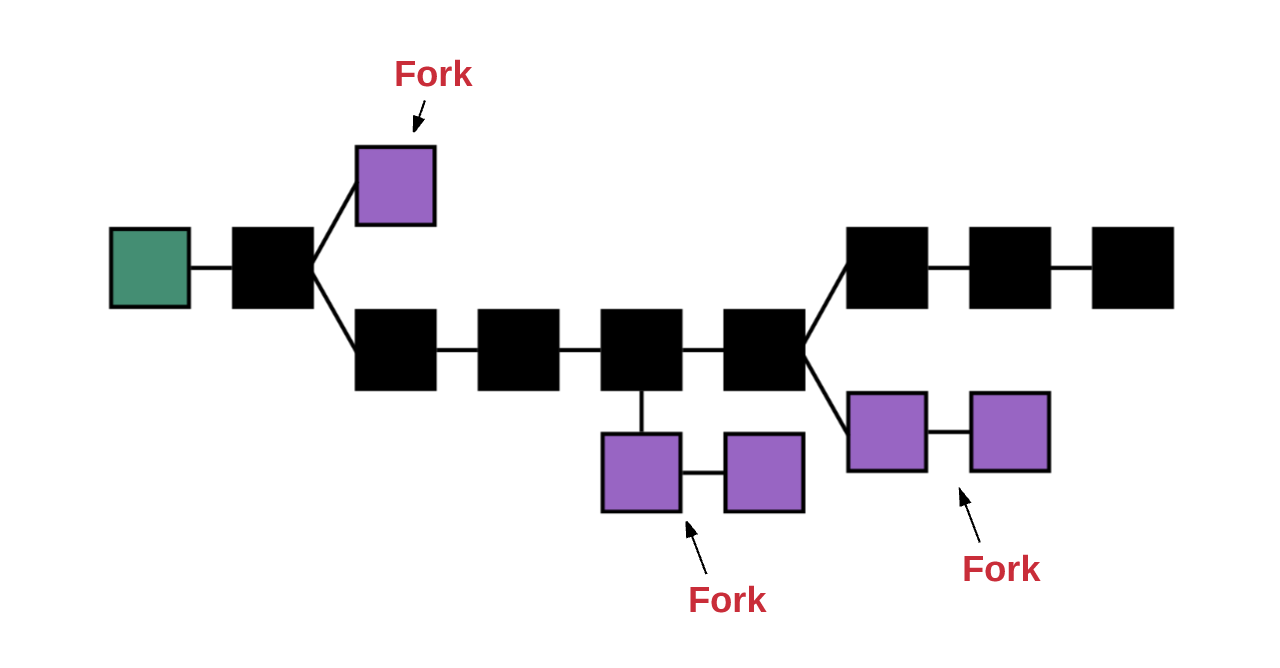
\includegraphics[scale=0.3]{scheme_4}
    \caption{Невозможная ситуация, существование несколькиз версий цепочек блоков.}
    \label{fig:scheme_4}
\end{figure}

Чтобы определить, какой из возможных путей является корректным, и предотвратить образования множества цепей, в Эфириуме применяется метод, называемый «протокол GHOST».

GHOST – «Жадное-и-Самое-Весомое-из-Известных-Дочерних-Деревьев» (Greedy Heaviest Observed Subtree)

Попробую объяснить простыми словами: протокол GHOST объявляет, что мы должны выбрать только тот путь, на котором было выполнено наибольшее число вычислений. Для определения такого пути можно использовать номер того блока, который был определен последним («листовой блок»). Благодаря такому подходу можно определить общее число блоков, находящихся в текущем пути (без учета блока первоначального состояния). Чем выше находится блок, тем длиннее путь и тем больше обоснований должны предоставить майнеры. Исходя из таких соображений, принимается единственно верная версия для текущего состояния. 

Теперь, когда вы уже имеете представление о том, что такое блокчейн, я предлагаю разобраться с основными компонентами, из которых состоит система Ethereum:

\begin{itemize}
 \item учетные записи 
 \item состояние
 \item горючее о вознаграждение
 \item транзакции
 \item блоки
 \item выполнение транзакций
 \item майнинг
 \item обоснование
\end{itemize}

Небольшое отступление перед тем, как мы начнем: при упоминании хэша X имеется ввиду хэш 
\href{https://ethereum.stackexchange.com/questions/550/which-cryptographic-hash-function-does-ethereum-use}{KECCAK-256}, используемый в Эфириуме.

\subsection{Учетные записи}

Глобальное общее состояние платформы Эфириум состоит из множества небольших объектов – учетных записей, которые взаимодействуют между собой за счет парадигмы обмена сообщениями. У каждой учетной записи есть определенное состояние и 20-байтовый адрес. Адресом в Эфириум является 160-битный идентификатор, используемый для идентификации любой из учетных записей (Рис. 5).

Всего существует два вида учетных записей:

\begin{itemize}
 \item Внешние учетные записи, контролируются с помощью закрытых ключей. При этом такие записи не имеют никакого кода, связанного с ними.
 \item Контрактные учетные записи, контролируются специальным кодом, указанным в условиях контракта, и имеющие связанный с ними код.
\end{itemize}


\begin{figure}
    \centering
    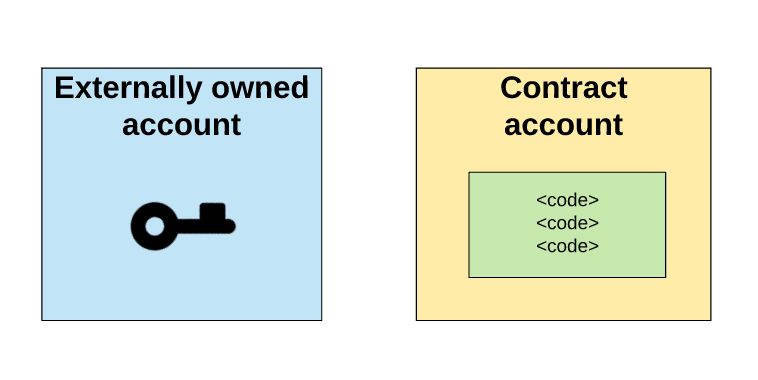
\includegraphics[scale=0.4]{scheme_5}
    \caption{Виды учетных записей.}
    \label{fig:scheme_5}
\end{figure}

\subsubsection{Внешние и контрактные учетные записи}

Давайте разберемся с основными отличиями между внешними и контрактными учетными записями. Для внешней учетной записи предусмотрена возможность отправлять сообщения другим внешним учетным записям, а также другим контрактным учетным записям. Для данной цели необходимо создать и зарегистрировать новую транзакцию, используя закрытый ключ. Сообщение между двумя внешними учетными записями является всего лишь значением для передачи. С другой стороны, сообщение, отправленное от внешней учетной записи к контрактной, подразумевает активацию кода контрактной учетной записи, при этом появляется возможность совершения определенных действий (например, с помощью такого сообщения можно переводить токены, записывать значения во встроенную память, создавать токены, выполнять некоторые вычисления, создавать новые контракты и т. д.). 

С помощью контрактных учетных записей, в отличие от внешних, самостоятельно инициировать новые транзакции невозможно. Вместо этого с помощью контрактных учетных записей можно только запускать транзакции в ответ на другие полученные транзакции (например, полученные из внешней учетной записи или из другой контрактной учетной записи). Более подробно о вызовах между контрактными учетными записями мы остановимся в разделе «Транзакции и сообщения» (Рис. 6).


\begin{figure}
    \centering
    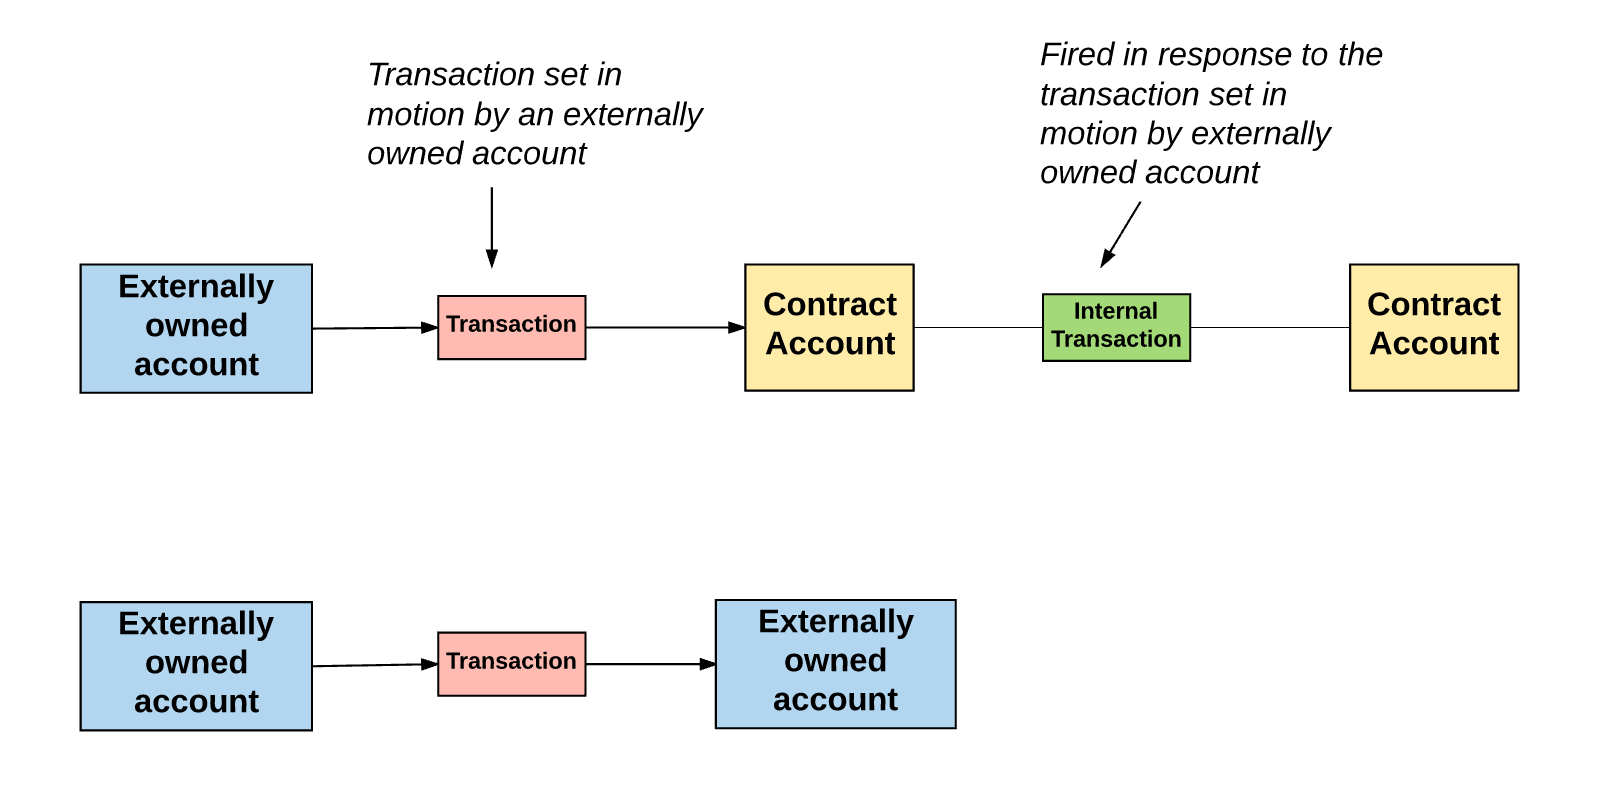
\includegraphics[scale=0.3]{scheme_6}
    \caption{Схема общения в зависимости от типа аккаунта.}
    \label{fig:scheme_6}
\end{figure}

Каждое действие в блокчейне Эфириума происходит благодаря транзакциям, инициируемым внешне контролируемыми учетными записями (Рис. 7). 


\begin{figure}
    \centering
    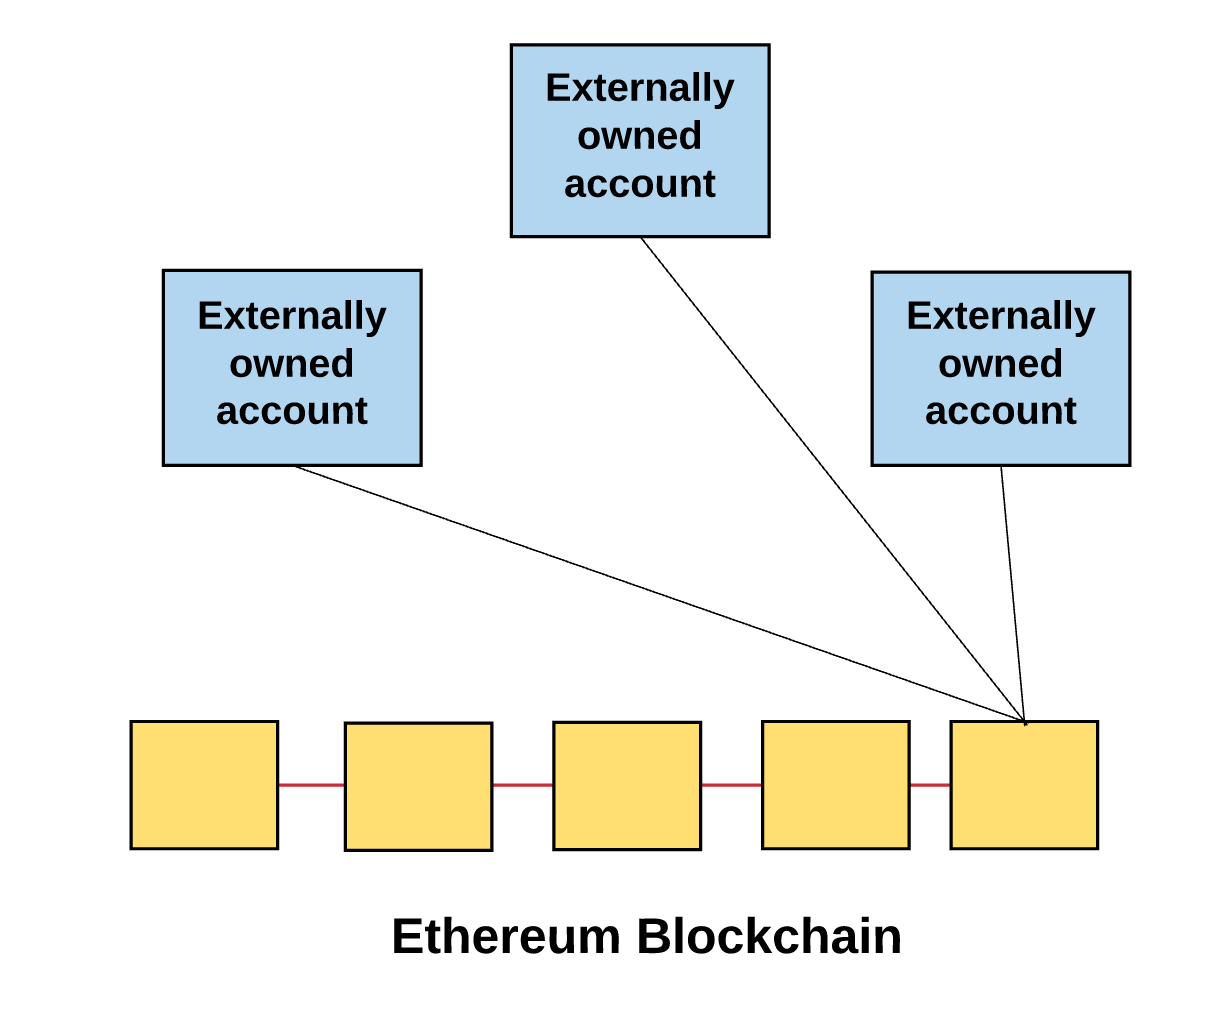
\includegraphics[scale=0.25]{scheme_7}
    \caption{Схема общения в зависимости от типа аккаунта.}
    \label{fig:scheme_7}
\end{figure}

\subsubsection{Состояние учетных записей}

Состояние каждой из учетных записей, вне зависимости от их типа, может принимать одно из четырех значений: 

\begin{itemize}
 \item nonce: Если настоящая учетная запись соответствует внешней учетной записи, то полученное число представляет собой количество транзакций, которые были отправлены с адреса учетной записи. Если учетная запись является контрактной учетной записью, то элемент nonce – это количество контрактов, созданных в данной учетной записи.
 \item balance: общее количество wei, приобретенных данной учетной записью. Например, каждый эфир, который является обменной единице Эфириума, содержит $10^{18}$ wei – дробных частей эфира.
 \item storageRoot: хэш корневого узла префиксного дерева Меркла (что собой представляет дерево Меркла мы рассмотрим немного позже). Дерево Меркла кодирует хэш содержимого данной учетной записи, при этом по умолчанию оно является пустым.
 \item codeHash: хэш EVM-кода (от англ. Ethereum Virtual Machine; что это такое я расскажу немного позже) учетной записи. Для контрактных учетных записей данное поле является кодом, который хэшируется и хранится в виде codeHash.
 
\end{itemize}

\begin{figure}
    \centering
    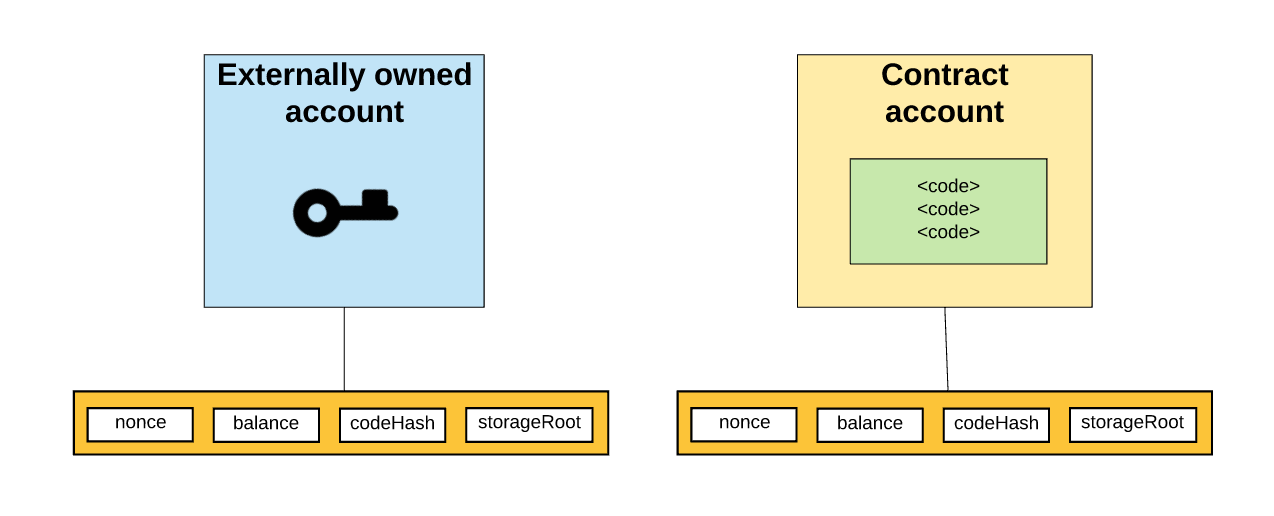
\includegraphics[scale=0.25]{scheme_8}
    \caption{Состояния учетных записей.}
    \label{fig:scheme_8}
\end{figure}


\subsubsection{Общее состояние системы}

Итак, мы разобрались, что глобальное состояние Эфириума – это сопоставление адресам учетной записи состояний счета. Это сопоставление хранится в структуре данных – префиксного дерева Меркла.

Дерево Меркла (или «Merkle trie») представляет собой тип двоичного файла, состоящего из набора узлов, которые включают:

\begin{itemize}
 \item определенное количество листовых узлов, которые располагаются в нижней части дерева, содержащего базовые данные
 \item набор промежуточных узлов, при этом каждый узел представляет собой хэш двух его дочерних узлов
 \item один корневой узел, также образованный из хэша двух дочерних узлов, который представляет вершину дерева
\end{itemize}


\begin{figure}
    \centering
    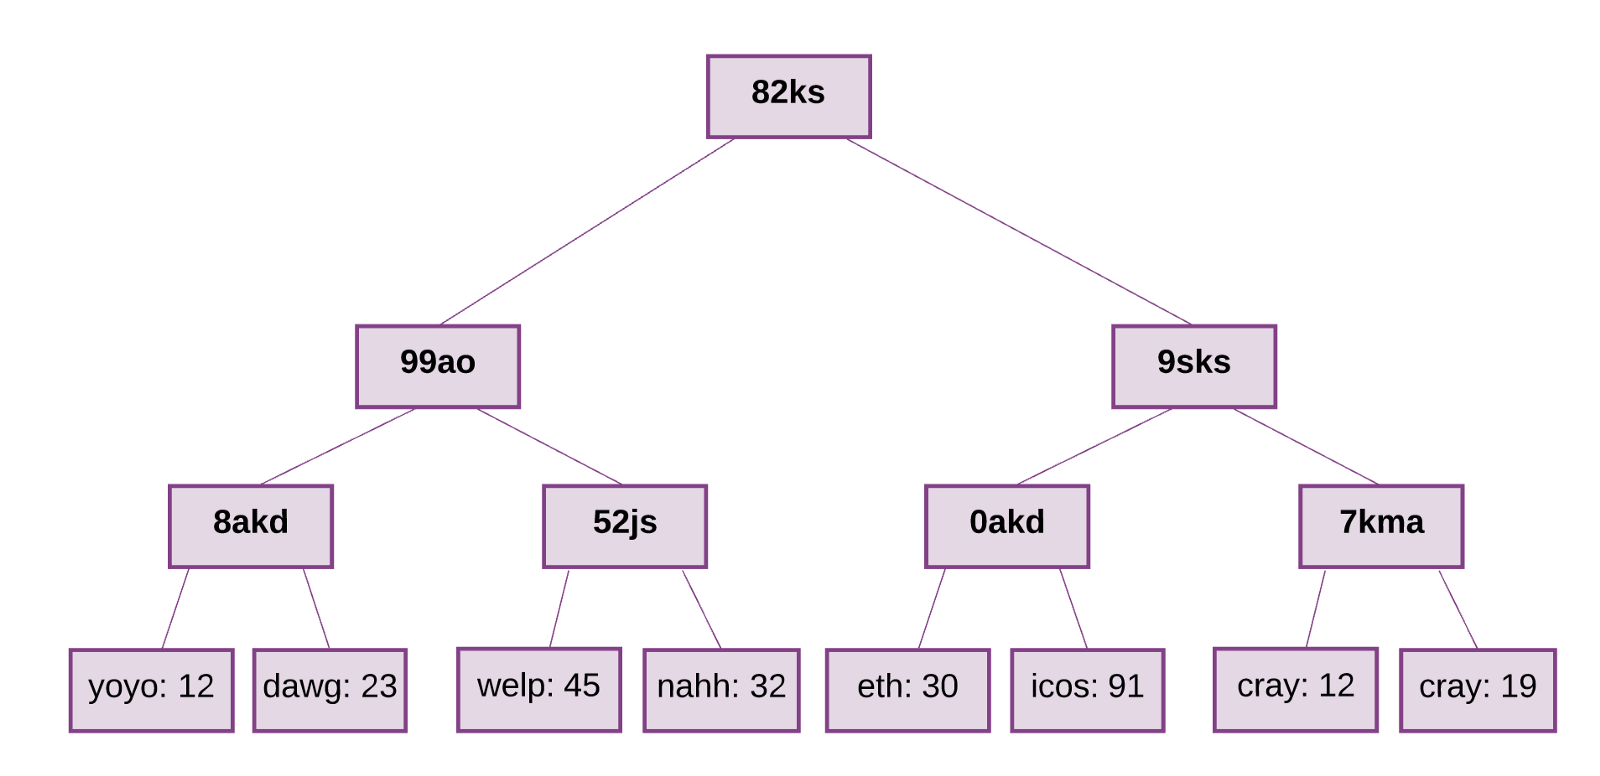
\includegraphics[scale=0.25]{scheme_9}
    \caption{Префиксное дерево Маркла.}
    \label{fig:scheme_9}
\end{figure}
















\begin{thebibliography}{9}

	\bibitem{lamport94}
	  \emph{Как работает Эфириум (Ethereum)?}
	  https://habr.com/post/407583/

\end{thebibliography}

\end{document}